\noindent
\begin{minipage}[t]{0.26\textwidth}
    \vspace{3.94cm}
    \noindent
    \textbf{\textsf{HÌNH 3}}\\
    {\small $f(x) = x^3$ là đơn ánh.}

    \vspace{2.3cm}
    \noindent
    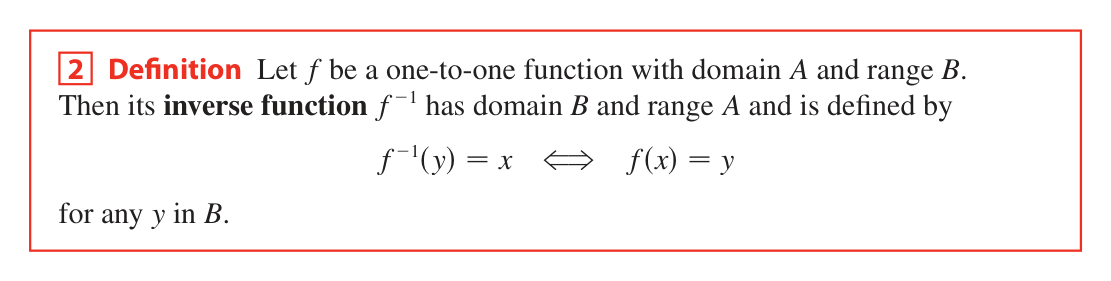
\includegraphics[width=\linewidth]{images/p0090_fig2.png}

    \vspace{0.12cm}
    \noindent
    \textbf{\textsf{HÌNH 4}}\\
    {\small $g(x) = x^2$ không phải là đơn ánh.}

    \vspace{1.48cm}
    \noindent
    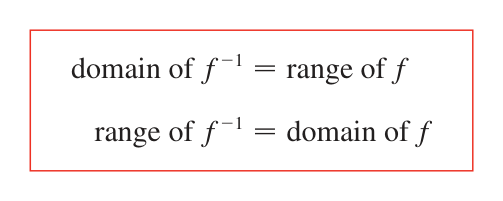
\includegraphics[width=0.92\linewidth]{images/p0090_fig3.png}

    \vspace{0.12cm}
    \noindent
    \textbf{\textsf{HÌNH 5}}

    \vspace{2.87cm}
    \noindent
    {\small Nghịch đảo $1/f(x)$ có thể được viết là $[f(x)]^{-1}$.}
\end{minipage}%
\hfill
\begin{minipage}[t]{0.71\textwidth}
    \noindent
    \textbf{\textsf{\color{stewartcyan}VÍ DỤ 1}}\quad Hàm số $f(x) = x^3$ có phải là đơn ánh không?

    \vspace{0.2cm}
    \noindent
    \textbf{\textsf{\color{stewartcyan}LỜI GIẢI 1}}\quad Nếu $x_1 \neq x_2$ thì $x_1^3 \neq x_2^3$ (hai số khác nhau không thể có cùng lập phương). Do đó, theo Định nghĩa 1, $f(x) = x^3$ là một hàm đơn ánh.

    \vspace{0.2cm}
    \noindent
    \textbf{\textsf{\color{stewartcyan}LỜI GIẢI 2}}\quad Từ Hình 3, ta thấy không có đường thẳng nằm ngang nào cắt đồ thị hàm số $f(x) = x^3$ nhiều hơn một lần. Vì vậy, theo Kiểm tra đường nằm ngang, $f$ là hàm đơn ánh.

    \vspace{0.08cm}
    \begin{flushright}
        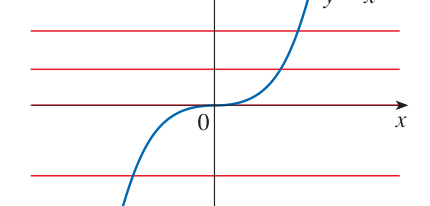
\includegraphics[width=0.46\textwidth]{images/p0090_fig1.png}\quad
        \raisebox{0.4cm}{\color{stewartcyan}$\blacksquare$}
    \end{flushright}

    \vspace{0.16cm}
    \noindent
    \textbf{\textsf{\color{stewartcyan}VÍ DỤ 2}}\quad Hàm số $g(x) = x^2$ có phải là hàm đơn ánh không?

    \vspace{0.2cm}
    \noindent
    \textbf{\textsf{\color{stewartcyan}LỜI GIẢI 1}}\quad Hàm số này không phải là đơn ánh vì chẳng hạn,
    \[
    g(1) = 1 = g(-1)
    \]
    và do đó $1$ và $-1$ có cùng một giá trị đầu ra.

    \vspace{0.16cm}
    \noindent
    \textbf{\textsf{\color{stewartcyan}LỜI GIẢI 2}}\quad Từ Hình 4, ta thấy có những đường thẳng nằm ngang cắt đồ thị của $g$ nhiều hơn một lần. Vì vậy, theo Kiểm tra đường nằm ngang, $g$ không phải là hàm đơn ánh. \hfill{\color{stewartcyan}$\blacksquare$}

    \vspace{0.33cm}
    \noindent
    Các hàm đơn ánh rất quan trọng vì chúng chính là những hàm số có hàm ngược tương ứng theo định nghĩa sau đây.

    \vspace{0.25cm}
    \begin{definitionbox}
        \textbf{\textsf{\color{stewartred}2\quad Định nghĩa}}\quad Cho $f$ là một hàm đơn ánh có tập xác định là $A$ và tập giá trị là $B$. Khi đó \textbf{hàm ngược} của nó, ký hiệu là $f^{-1}$, có tập xác định là $B$ và tập giá trị là $A$, được xác định bởi
        \[
        f^{-1}(y) = x \quad\Longleftrightarrow\quad f(x) = y
        \]
        với mọi $y$ thuộc $B$.
    \end{definitionbox}

    \vspace{0.29cm}
    \noindent
    Định nghĩa này phát biểu rằng nếu $f$ ánh xạ $x$ thành $y$, thì $f^{-1}$ sẽ ánh xạ $y$ trở lại thành $x$. (Nếu $f$ không phải là đơn ánh, thì $f^{-1}$ sẽ không được xác định một cách duy nhất.) Sơ đồ mũi tên ở Hình 5 chỉ ra rằng $f^{-1}$ đảo ngược tác động của $f$. Lưu ý rằng
    \begin{center}
        \begin{definitionbox}
            \centering
            \begin{tabular}{rcl}
                tập xác định của $f^{-1}$ & $=$ & tập giá trị của $f$ \\[5pt]
                tập giá trị của $f^{-1}$ & $=$ & tập xác định của $f$
            \end{tabular}
        \end{definitionbox}
    \end{center}

    \vspace{0.2cm}
    \noindent
    Ví dụ, hàm ngược của $f(x) = x^3$ là $f^{-1}(x) = x^{1/3}$ bởi vì nếu $y = x^3$, thì
    \[
    f^{-1}(y) = f^{-1}(x^3) = (x^3)^{1/3} = x
    \]

    \vspace{0.16cm}
    \noindent
    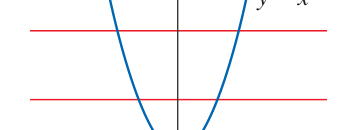
\includegraphics[height=1.05em,trim=0 0 0 0]{images/p0090_fig4.png}\ \textbf{\textsf{\color{stewartred}LƯU Ý}}\quad {\color{stewartred}Không được nhầm lẫn số $-1$ trong ký hiệu $f^{-1}$ với một số mũ. Do đó}
    \[
    {\color{stewartred}f^{-1}(x) \quad\text{\textit{không có nghĩa là}}\quad \frac{1}{f(x)}}
    \]
\end{minipage}